\chapter{System Maintenance}

\section{Environment}

\subsection{Software}
The software and modules I used to implement the program:
\begin{itemize}
	\item Python 3
	\item IDLE
	\item PyQt 4
	\item SQLite3
	\item Notepad++
	\item SQLiteInspecter
\end{itemize}

\subsection{Usage Explanation}
\begin{center}
	\begin{tabular}{|p{3cm}|p{6cm}|}
		\hline
		\textbf{Software}   & \textbf{Explanation for use of software} \\ \hline
		Python 3 & I know this language well and python is a relatively powerful language. Python allows bug finding and fixing to be incredibly easy as the program can be compiled quickly as you write it instead of using a separate compiler. Python is free and is object orientated. \\ \hline
		IDLE &  I used this python environment as it comes with the basic installation of python and is the only editor installed on school computers. \\ \hline
		PyQt4 & PyQt allows for the easy creation of a GUI. \\ \hline
		SQLite3 & Used for database creation and editing as I have been taught this and SQL allows for easy database manipulation. \\ \hline
		Notepad++ & Used for the creation of HTML files as I know how to use it and HTML files can be run from the program. \\ \hline
		SQLiteInspector & I used this program that my teacher created to test SQL queries and to check data is added to the database properly. \\ \hline
	\end{tabular}
\end{center}


\subsection{Features Used}

\subsubsection{Python 3}

\begin{itemize}
	\item I could create a basic CLI program to make sure my logic and usability was good before creating a GUI program. 
	\item Object orientated.
	\item Many modules pre-installed and many that can be installed.
	\item We have been learning this programing language for the majority of our school year.
	\item The cx\_Freeze module can be used to create a .exe file.
\end{itemize}

\subsubsection{Idle}

\begin{itemize}
	\item IDLE displays python code in coloured syntax showing where mistakes have been made and makes it easier to fix errors quickly.
	\item Is an interpreter so the program is run very quickly and errors can be located easily 
	\item Useful shortcuts such as Ctrl+C for copy, F5 to run and Ctrl+F for find.
	\item You can right click errors to locate and highlight the line causing the problem.
\end{itemize}

\subsubsection{PyQt4}

\begin{itemize}
	\item Easy to install.
	\item Many types of widgets to use.
	\item Can utilise SQLite3
	\item Has good documentation on sourceforge.
\end{itemize}

\subsubsection{SQLite3}

\begin{itemize}
	\item Used for database creation and editing.
	\item I have been taught this in class.
	\item Allows for easy database manipulation.
\end{itemize}

\subsubsection{Notepad++}

\begin{itemize}
	\item Used for the creation of HTML files.
	\item I know how to use it.
	\item HTMl files can be compiled from the program.
	\item Coloured syntax for HTML.
\end{itemize}

\subsubsection{SQLiteInspector}

\begin{itemize}
	\item Used for viewing databases and tables.
	\item Used for testing queries that act on the database without having to run the python program.
\end{itemize}

\section{System Overview}

%use as many subsections as necessary for the system components
\subsection{Logging In}
The login screen has the purpose of protecting sensitive data and adding an extra layer of security. The user must supply a username and a password. When the accept button is clicked the program compares the username and password the user supplied with those stored on an encrypted binary file. The username and password are hard-coded and cannot be changed due to the fact there is only one user.

\subsection{Graphical User Interface}
The GUI uses a simple design that should make the usage of the program easy to comprehend and visualise. The program is easily navigable via the menu bar and the task bar. Data is input using combo boxes and line edits or directly edited via the table display. All buttons are properly labeled and all functions can be accessed from the taskbar.

\subsection{Viewing Data}
The program displays all the data in the table selected which can then be searched or sorted. Almost all the windows of the GUI display the table of the data type.

\subsection{Adding Data}
Data is added to the database via line edits and combo boxes. The line edits are validated by the box being green if valid, red if invalid or amber if incomplete but still valid. Any data added via the combo-boxes will always be valid as only valid dates can be selected. An accept button must be pressed before the data is actually added to the database.

\subsection{Editing Data}
Data is edited directly in the table that is displayed. Single click on the field being edited and input the new data, then press Enter when done and the database will be changed. The table can be sorted in the editing screen to locate the entities that need to be edited.

\subsection{Deleting Data}
The table in the deleting windows can be sorted to find the correct entities. Double clicking on a row will delete the entity that row corresponds to.

\subsection{Printing Invoices}
Clicking on the print invoices button will bring up a window with the ability to select a date to print all the invoices from.


\section{Code Structure}

%use as many subsections as necessary for the code sections
\subsection{Overview}
My program utilises object orientated programing not only because this is the way PyQt operates but because OOP allows code to be reused or to be used more efficiently.


\subsection{Adding Data}

\pythonfile{./Implementation/AddData.py}

The AddData file contains a base EnterDataDialog class and two daughter classes for Parent and Member that extend and inherit from the base class. The base class contains common features between the two daughter classes such as many of the line edits. I have formatted the program this way so that more daughter classes that are similar to the base class can be created easily with no repeating code.

The AddData class is used to create a widget that is inserted into the central widget. The widget displays the table of the data type being added (Member, Parent or Invoice) and several line edits and combo-boxes for adding data. It also contains an accept button that needs to be pressed for the data in the line edits and combo-boxes to be added to the database. 


\subsection{Editing Data}

\pythonfile{./Implementation/EditData.py}

The EditData class is used to create a widget that is inserted into the central widget. The widget displays the table of the data type being edited (Member, Parent or Invoice). This table can be searched via entering text into the line edit above the table and clicking on a field and typing will enter new data into that field replacing the old one.


\subsection{Deleting Data}

\pythonfile{./Implementation/DeleteData.py}

The DeleteData class is used to create a widget that is inserted into the central widget. The widget displays the table of the data type being deleted (Member, Parent or Invoice). This table can be searched via entering text into the line edit above the table and double clicking on the row to be deleted will delete it.


\subsection{Validation}

\pythonfile[firstline=220,lastline=228]{./Implementation/AddData.py}

\pythonfile[firstline=44,lastline=47]{./Implementation/AddData.py}

This is an example of a validation function to validate the line edit add\_first\_name. The text is received from the line edit and if the data is text it is returned to the line edit capitalised so the text is all in the same format. Then the text is compared to a regular expression and if valid a True signal is returned. Then if the signal is true but the length of the text is under 11 (The length of a phone number) the line edit is set to amber, if it is true and long enough it is set to green and if untrue regardless of length then it is set to red.


\subsection{Login Box}

\pythonfile[firstline=1,lastline=40]{./Implementation/LoginBox.py}

The LoginBox class creates a popup-window with two line edits for a username and a password and a push button to check the data is correct.


\section{Main Function}

\pythonfile[firstline=544,lastline=547]{./Implementation/main_window.py}

This function initialises the application if the class is run as the main class.


\section{Variable Listing}
My orginal data dictionary:

\begin{center}
	\begin{longtable}{|p{2.5cm}|p{2.5cm}|p{2.5cm}|p{2.5cm}|l}
		\hline
		\textbf{Name}                    & \textbf{Data Type}    & \textbf{Length}                  & \textbf{Validation} \\ \hline
		MemberID                           & String            & 4 digits                & Numbers only \\ \hline
		ParentID                             & String            & 4 digits                & Numbers only \\ \hline
		Member first name              & String            & 1-20 characters   & Letters only \\ \hline
		Member last name               & String           &1-20 characters &  Letters only \\ \hline
		Parents first name               & String           & 1-20 characters &  Letters only \\ \hline
		Parent last name                 & String           & 1-20 characters &  Letters only \\ \hline
		Member town name                 & String           & 1-20 characters &  Letters only \\ \hline
		Member street name                 & String           & 1-20 characters &  Letters only \\ \hline
		Member house name/number & String              & 1-20 characters &  Letters only \\ \hline
		Parent town name                 & String           & 1-20 characters &  Letters only \\ \hline
		Parent street name                 & String           & 1-20 characters &  Letters only \\ \hline
		Parent house name/number & String                 & 1-20 characters &  Letters only \\ \hline
		Parent phone number         & Integer        & 12 digits & Numbers only, correct format and a valid phone number \\ \hline
		Parent email                        & String          & 1-30 characters &  Letters only \\ \hline
		Member date of birth          & Datetime       & 6 digits & Numbers only (dd/mm/yy) \\ \hline
		Invoice ID                           & Integer       & 4 digits & Numbers only \\ \hline
		Was invoice paid                 & Integer       & 4-6 digits & Numbers only, correct format and a valid date \\ \hline
		Date invoice was sent        & Datetime       & 6 digits & Numbers only (dd/mm/yy) \\ \hline
	\end{longtable}
\end{center}

My variable listing:

\begin{center}
	\begin{longtable}{|p{2cm}|p{2cm}|p{2cm}|p{2cm}|l}
		\hline
		\textbf{Variable}  &  \textbf{Use}  &  \textbf{Figure}  &  \textbf{Line Number} \\ \hline
		%Main Window
		username & Stores the username input from the user & \ref{main_window} & 131 \\ \hline
		password & Stores the password input from the user &  \ref{main_window} & 132 \\ \hline
		path & Stores the path of where the database is & \ref{main_window} & 156 \\ \hline
		query & Stores a query to be used in a QSqlQueryModel & \ref{main_window} & 244 \\ \hline
		index & Stores the index of the statement chosen in the ordering combobox & \ref{main_window} & 266 \\ \hline
		text & Stores text in the search box & \ref{main_window} & 362 \\ \hline
		filter\_query & Stores the sql filter to be added to a QSqlTableModel & \ref{main_window} & 363 \\ \hline
		row & Stores the row that has been double clicked & \ref{main_window} & 502 \\ \hline
		values & Stores the values returned from a function & \ref{main_window} & 539 \\ \hline
		%AddData
		updatedData & Stores a signal to be sent & \ref{add_data} & 9 \\ \hline
		pattern & Used to store a regular expression to compare to the text in a line edit & \ref{add_data} & 45 \\ \hline
		valid & Used to store the results of comparison of the text and the pattern & \ref{add_data} & 46 \\ \hline
		text & Stores text in the search box & \ref{add_data} & 50 \\ \hline
		valid & Stores the return value of the boolean result returned from the validate function & \ref{add_data} & 52 \\ \hline
		currentYear & Stores the current year & \ref{add_data} & 114 \\ \hline
		count & Starts at 0 and has 1 added to it each time the loop ends & \ref{add_data} & 117 \\ \hline
		day & Stores the day selected & \ref{add_data} & 140 \\ \hline
		month & Stores the month selected & \ref{add_data} & 141 \\ \hline
		year & Stores the year selected & \ref{add_data} & 142 \\ \hline
		dob & Stores a list of the day, month and year & \ref{add_data} & 149 \\ \hline
		values & Stores the values returned from a function & \ref{add_data} & 151 \\ \hline
		cursor & Stores the cursor & \ref{add_data} & 159 \\ \hline
		sql & Stores an sql statement & \ref{add_data} & 161 \\ \hline
		%DeleteData
		updatedData & Stores a signal to be sent & \ref{delete_data} & 8 \\ \hline
		values & Stores the values returned from a function & \ref{delete_data} &  \\ \hline
		%Create Database
		db\_name & Stores the name of the databse & \ref{create_database} & 3 \\ \hline
		table\_name & Stores the name of the table being affected & \ref{create_database} & 3 \\ \hline
		cursor & Stores the cursor & \ref{create_database} & 5 \\ \hline
		sql & Stores an sql statement & \ref{create_database} & 25 \\ \hline
		keep\_table & Stores a boolean of whether the user wants to keep the table or not & \ref{create_database} & 8 \\ \hline
		response & Stores an input of y or n from the user & \ref{create_database} &  10 \\ \hline
		termPrice & Stores the price of a term & \ref{create_database} & 81 \\ \hline
		siblingDiscountAmount & Stores the discount a sibling gets & \ref{create_database} & 82 \\ \hline
		values & Stores the values returned from a function & \ref{create_database} & 84 \\ \hline
		%Login Box
		username & Stores the username input from the user & \ref{login_box} & 15 \\ \hline
		password & Stores the password input from the user &  \ref{login_box} & 16 \\ \hline
		%ManageInvoices
		updatedData & Stores a signal to be sent & \ref{manage_invoices} & 8 \\ \hline
		currentYear & Stores the current year & \ref{manage_invoices} & 44 \\ \hline
		count & Starts at 0 and has 1 added to it each time the loop ends & \ref{manage_invoices} & 46 \\ \hline
		day & Stores the day selected & \ref{manage_invoices} & 72 \\ \hline
		month & Stores the month selected & \ref{manage_invoices} & 73 \\ \hline
		year & Stores the year selected & \ref{manage_invoices} & 74 \\ \hline
		date & Stores the year, month and day combined & \ref{manage_invoices} & 81
		values & Stores the values returned from a function & \ref{manage_invoices} & 83 \\ \hline
		cursor & Stores the cursor & \ref{manage_invoices} & 88 \\ \hline
		sql & Stores an sql statement & \ref{manage_invoices} & 90 \\ \hline
		addData & Stores a signal to be sent  & \ref{manage_invoices} & 124 \\ \hline
		deleteData & Stores a signal to be sent  & \ref{manage_invoices} & 125\\ \hline
		%SendInvoices
		name & Stores a name for the html file & \ref{send_invoices} & 23 \\ \hline
		html & Stores a large string that a html file will be created from & \ref{send_invoices} & 25 \\ \hline
		html & Stores a large string that a html file will be created from that has been returned from a function & \ref{send_invoices} & 75 \\ \hline
		values & Stores the values returned from a function & \ref{send_invoices} & 125 \\ \hline
		%SortingTable
		items & Stores a list of items to be added to a combo-box & \ref{sorting_table} & 33 \\ \hline
		%StyleSheet
		css & Stores a large string of a cascading style sheet & \ref{style_sheet} & 1 \\ \hline
	\end{longtable}
\end{center}




\section{System Evidence}

\subsection{User Interface}

\subsubsection{Login Screen}
\begin{figure}[H]
\includegraphics[width=\textwidth]{./Maintenance/Images/LoginScreen.png}
    \caption{Login Screen} \label{fig:login_screen}
\end{figure}

Displays when the program is run. The login pop-up contains two line edits to input the username and password, two labels labeling the line edits, a label desciping the purpose of the login pop-up and an enter button. When the correct username and password are entered the main program shows.

\begin{figure}[H]
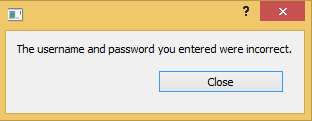
\includegraphics[width=\textwidth]{./Maintenance/Images/LoginScreenIncorrect.png}
    \caption{Pop-up when login details are incorrect} \label{fig:login_screen_incorrect}
\end{figure}

Displays when the username and password are incorrect. Contains a label with information and a button to close the window.

\subsubsection{Displaying Tables}
\begin{figure}[H]
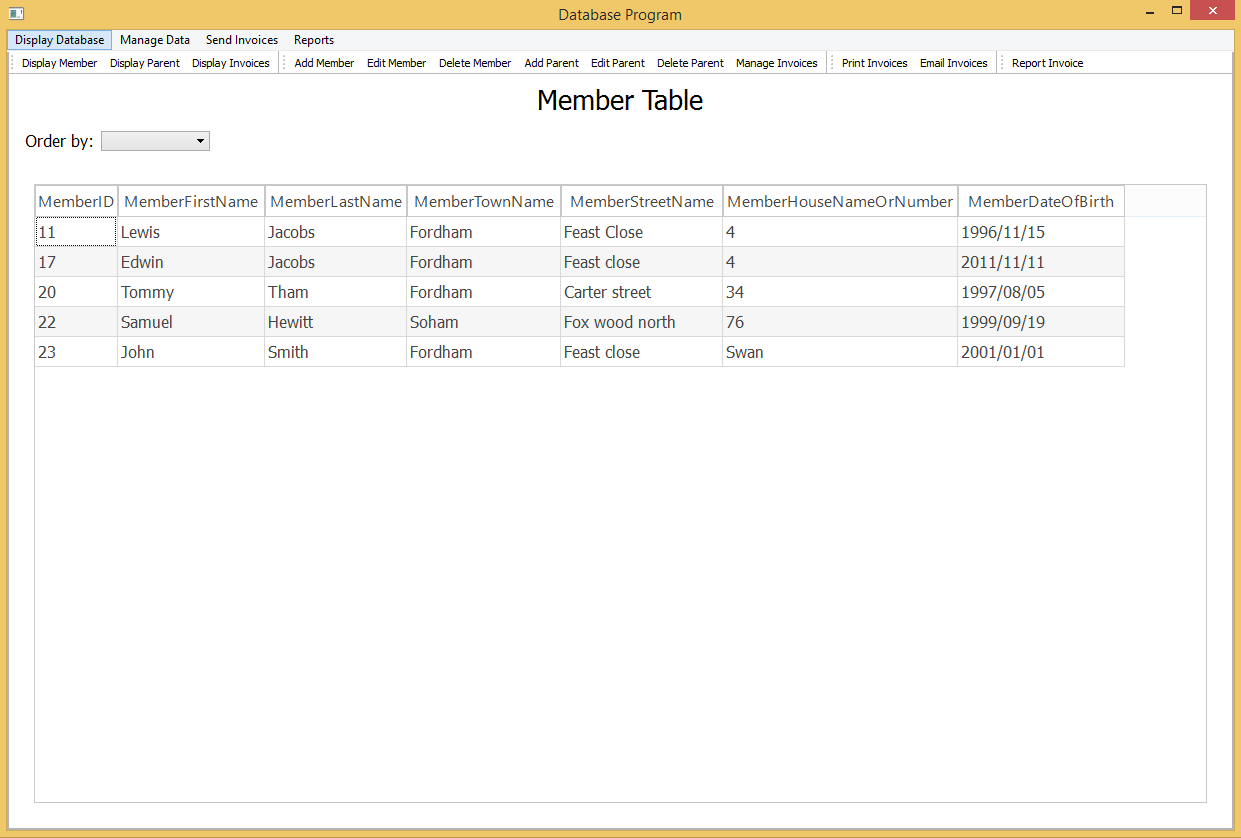
\includegraphics[width=\textwidth]{./Maintenance/Images/DisplayMember.png}
    \caption{Displaying Member} \label{fig:display_member}
\end{figure}

Displays after the login screen and when Display Member is clicked. Contains a label descriping the function of the screen, a table view displaying the Member table and a combobox to order the table.

\begin{figure}[H]
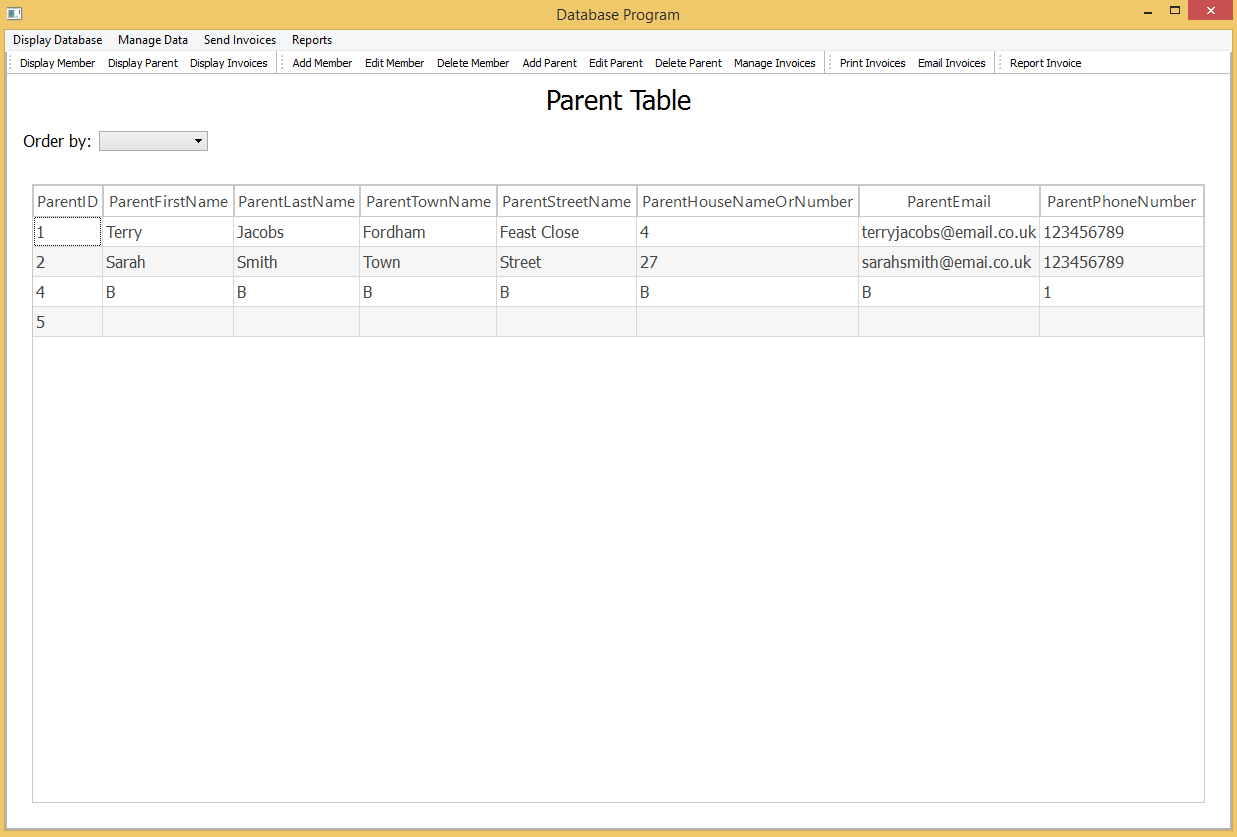
\includegraphics[width=\textwidth]{./Maintenance/Images/DisplayParent.png}
    \caption{Displaying Parent} \label{fig:display_parent}
\end{figure}

Displays when Display Parent is clicked. Contains a label descriping the function of the screen, a table view displaying the Parent table and a combobox to order the table.

\begin{figure}[H]
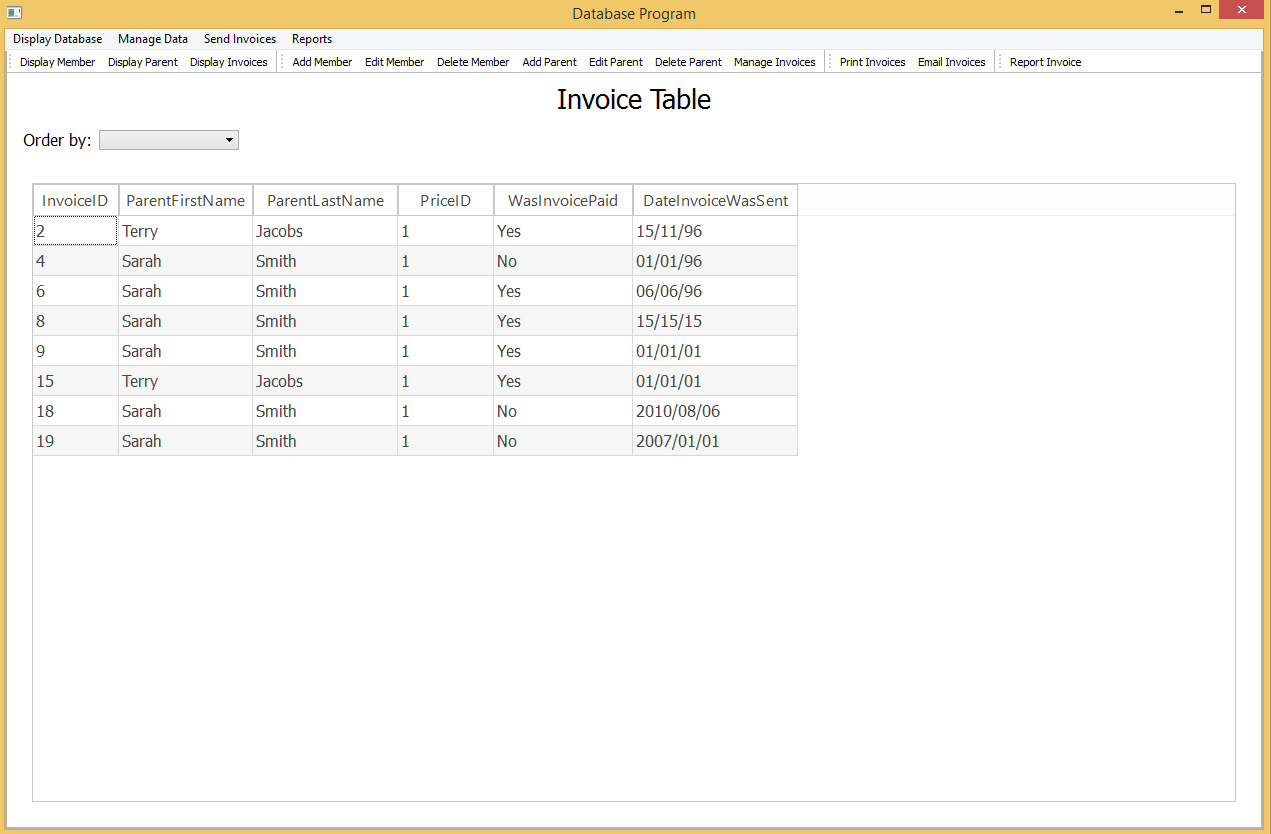
\includegraphics[width=\textwidth]{./Maintenance/Images/DisplayInvoice.png}
    \caption{Displaying Invoice} \label{fig:display_invoice}
\end{figure}

Displays when Display Invoice is clicked. Contains a label descriping the function of the screen, a table view displaying the Invoice table and a combobox to order the table.

\subsubsection{Adding Data}
\begin{figure}[H]
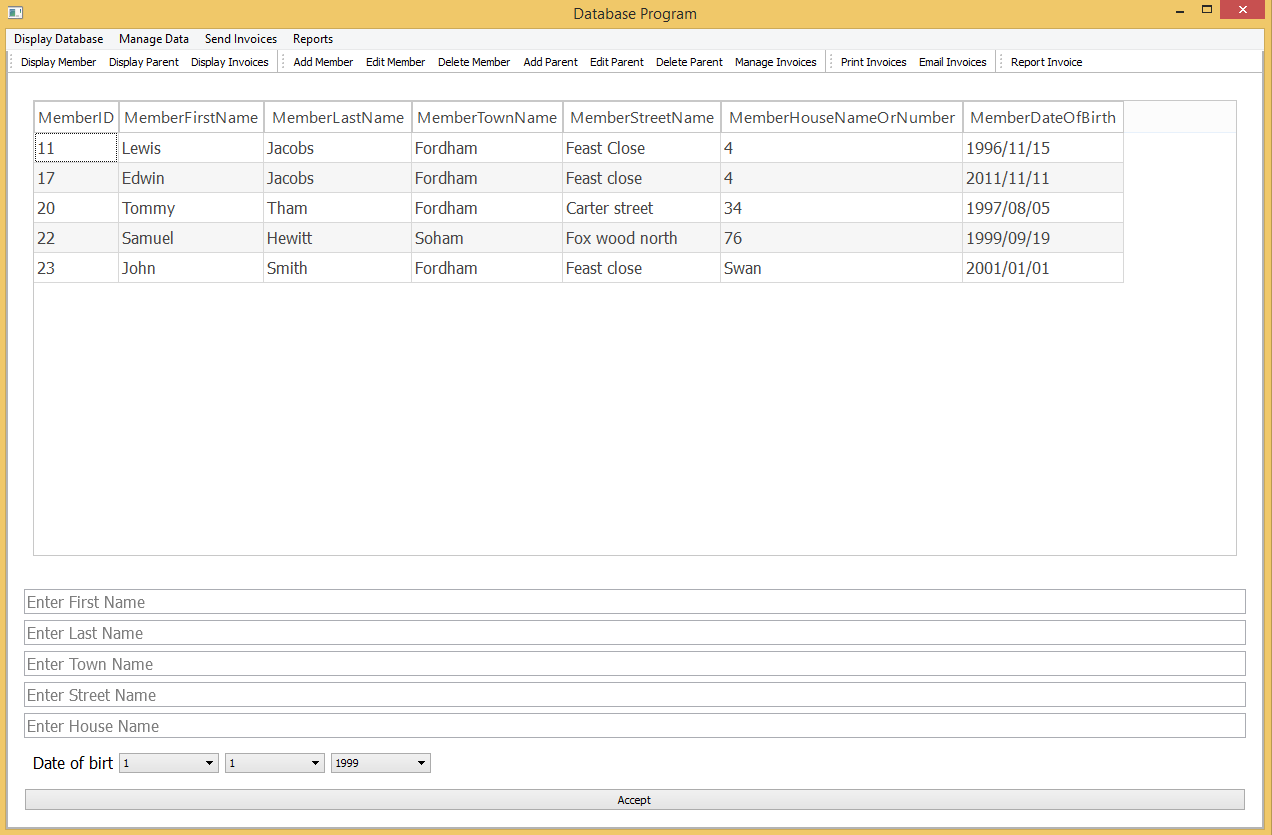
\includegraphics[width=\textwidth]{./Maintenance/Images/AddMember.png}
    \caption{Adding Member} \label{fig:add_member}
\end{figure}

Displays when Add Member is clicked. Contains a table view displaying the Member table and a series of linedits and comboboxes for the input of data into the table.

\begin{figure}[H]
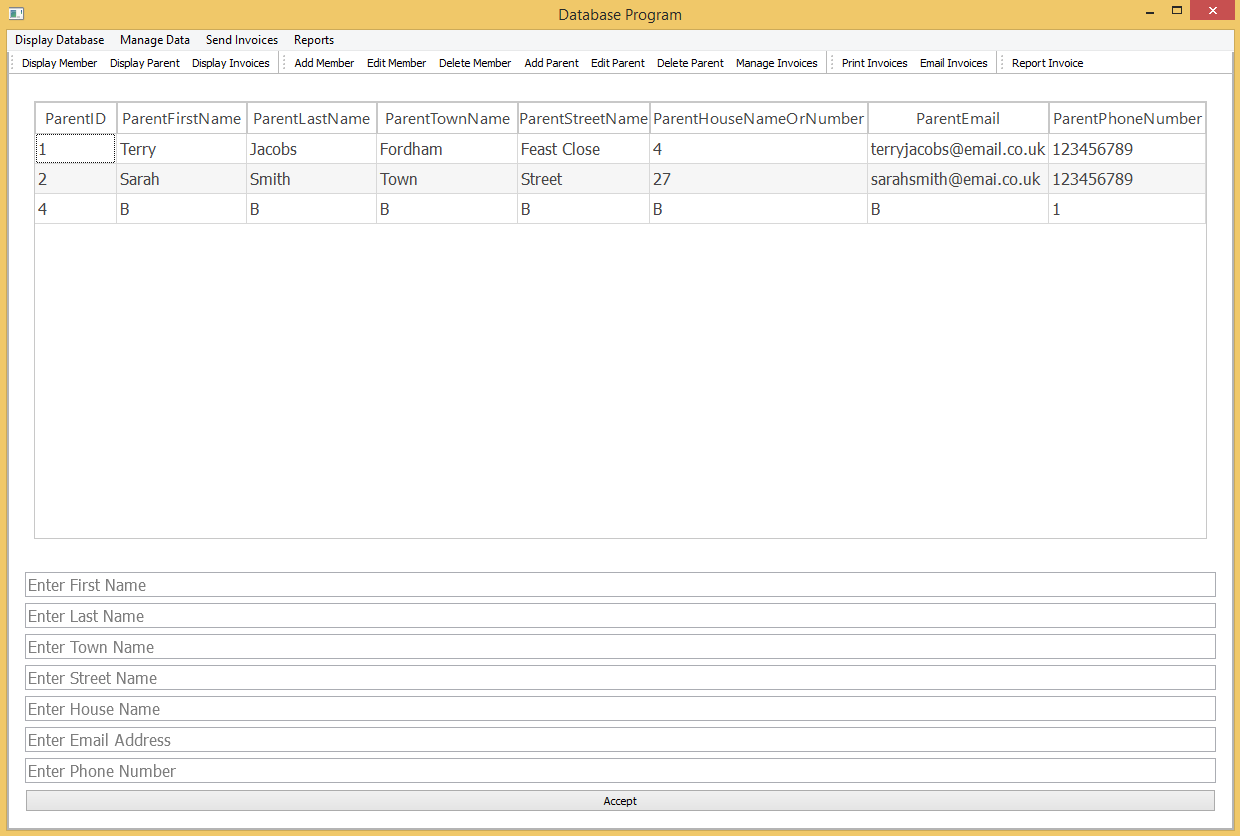
\includegraphics[width=\textwidth]{./Maintenance/Images/AddParent.png}
    \caption{Adding Parent} \label{fig:add_parent}
\end{figure}

Displays when Add Parent is clicked. Contains a table view displaying the Parent table and a series of linedits and comboboxes for the input of data into the table.

\subsubsection{Editing Data}
\begin{figure}[H]
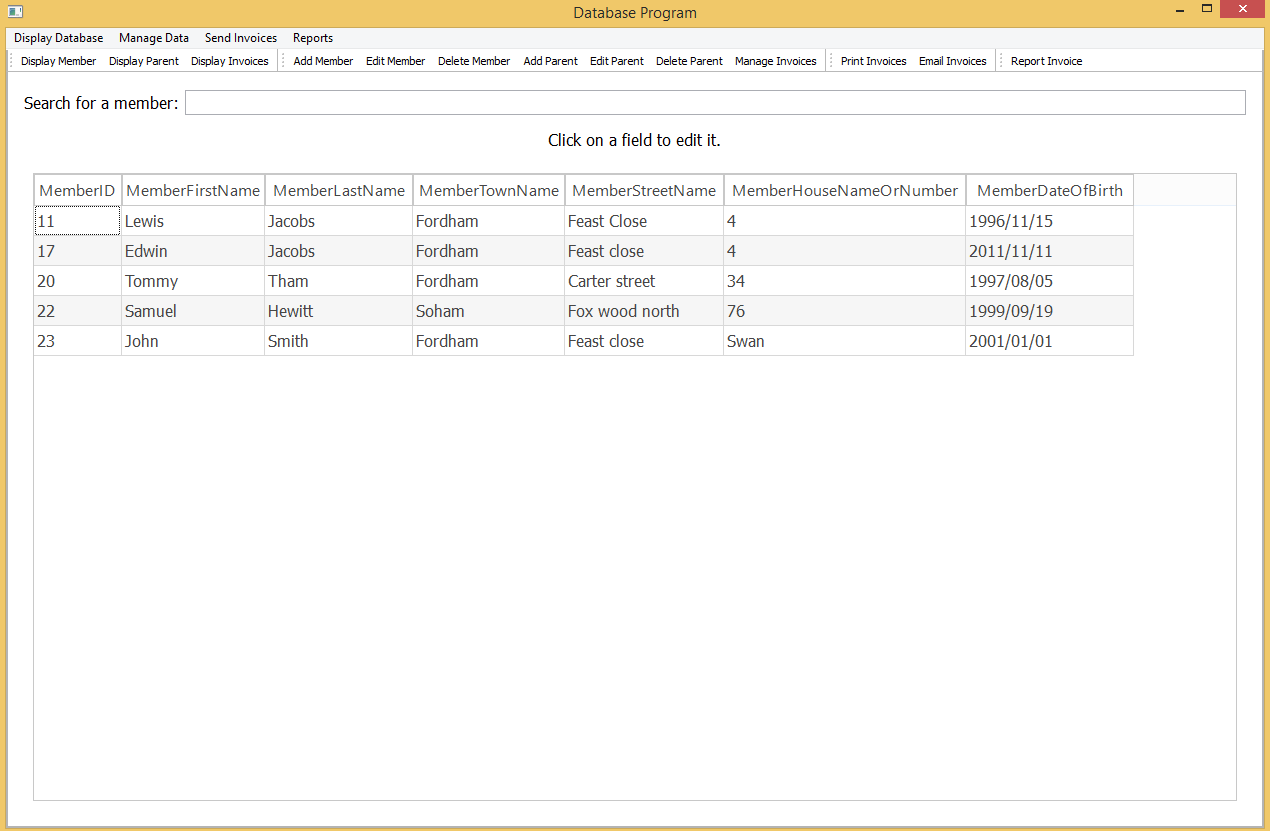
\includegraphics[width=\textwidth]{./Maintenance/Images/EditMember.png}
    \caption{Editing Member} \label{fig:edit_member}
\end{figure}

Displays when Edit Member is clicked. Contains an editable table view displaying the Member table and a linedit to search the table.

\begin{figure}[H]
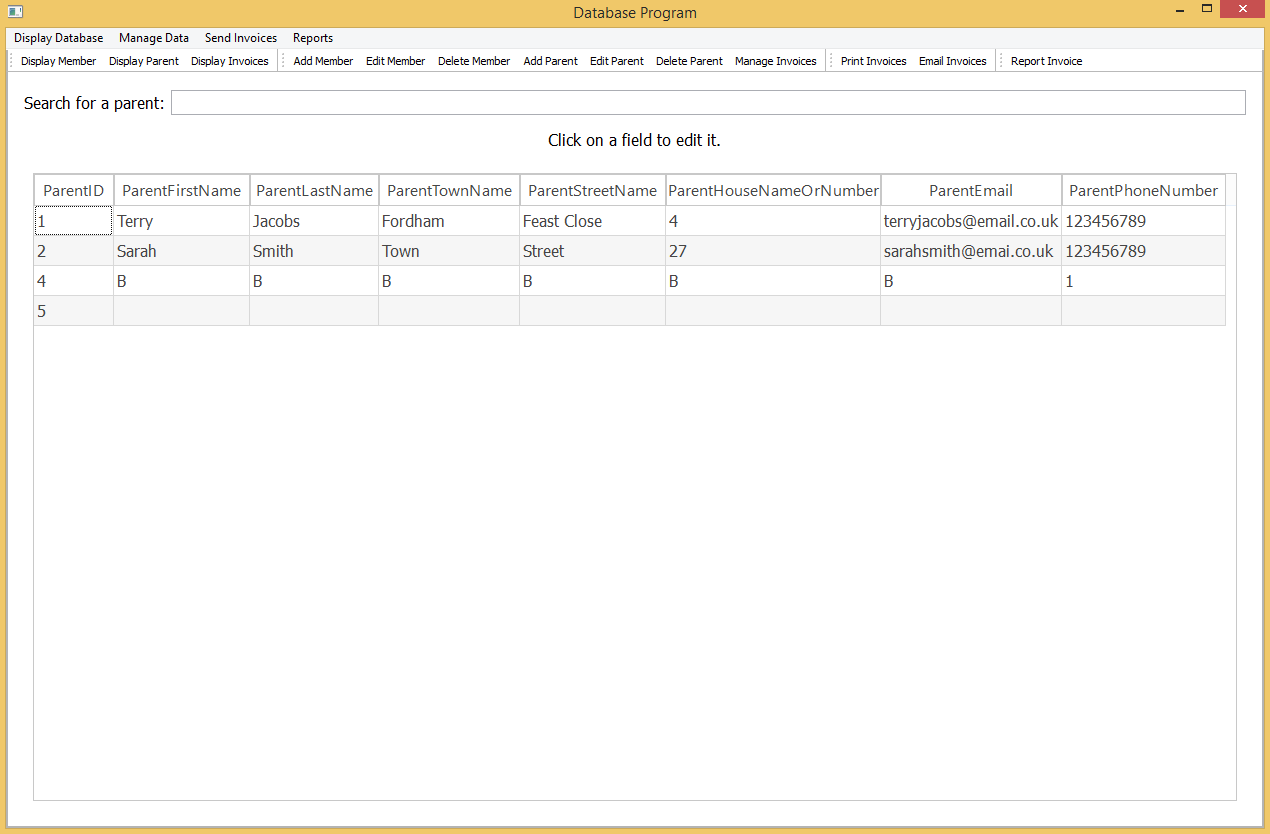
\includegraphics[width=\textwidth]{./Maintenance/Images/EditParent.png}
    \caption{Editing Parent} \label{fig:edit_parent}
\end{figure}

Displays when Edit Parent is clicked. Contains an editable table view displaying the Parent table and a linedit to search the table.

\subsubsection{Deleting Data}
\begin{figure}[H]
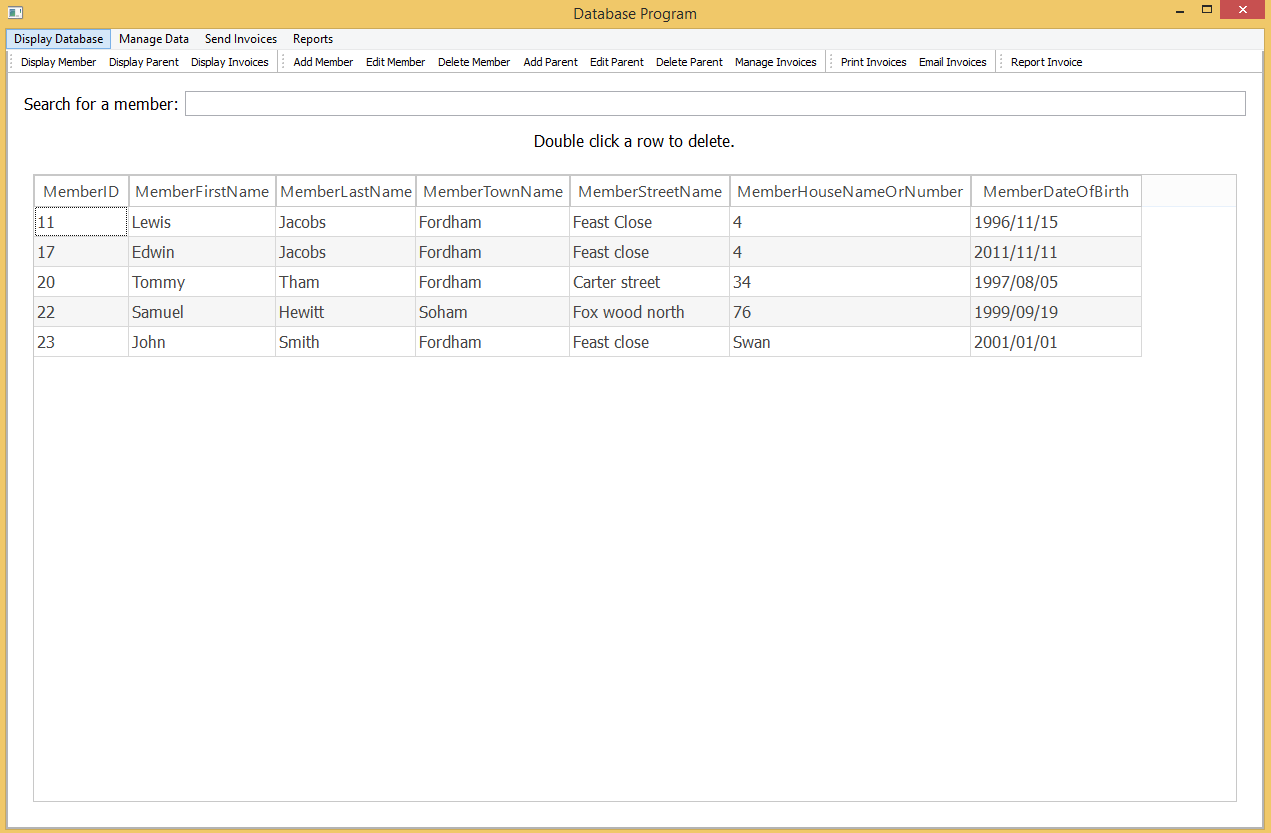
\includegraphics[width=\textwidth]{./Maintenance/Images/DeleteMember.png}
    \caption{Deleting Member} \label{fig:delete_member}
\end{figure}

Displays when Delete Member is clicked. Contains a table view displaying the Member table and a linedit to search the table.

\begin{figure}[H]
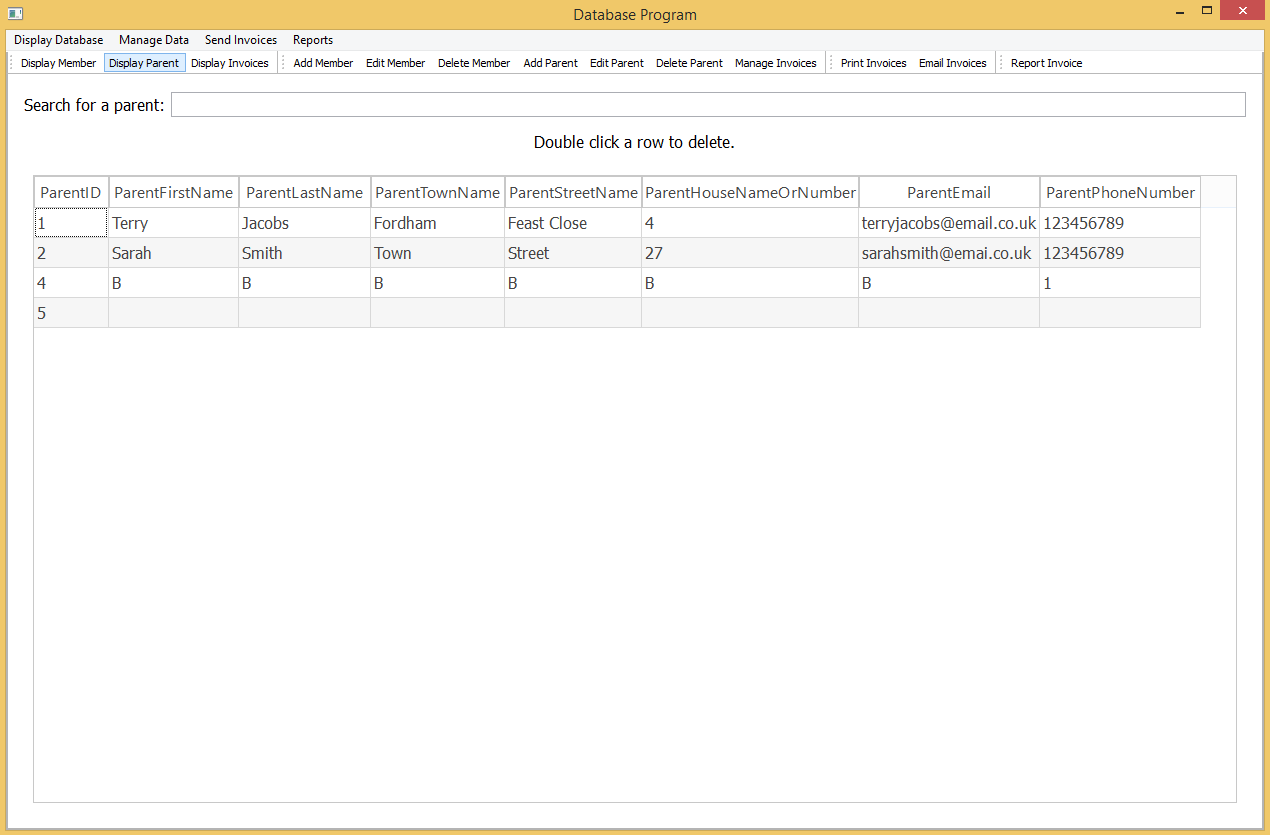
\includegraphics[width=\textwidth]{./Maintenance/Images/DeleteParent.png}
    \caption{Deleting Parent} \label{fig:delete_parent}
\end{figure}

Displays when Delete Parent is clicked. Contains a table view displaying the Parent table and a linedit to search the table.

\subsubsection{Managing Invoices}
\begin{figure}[H]
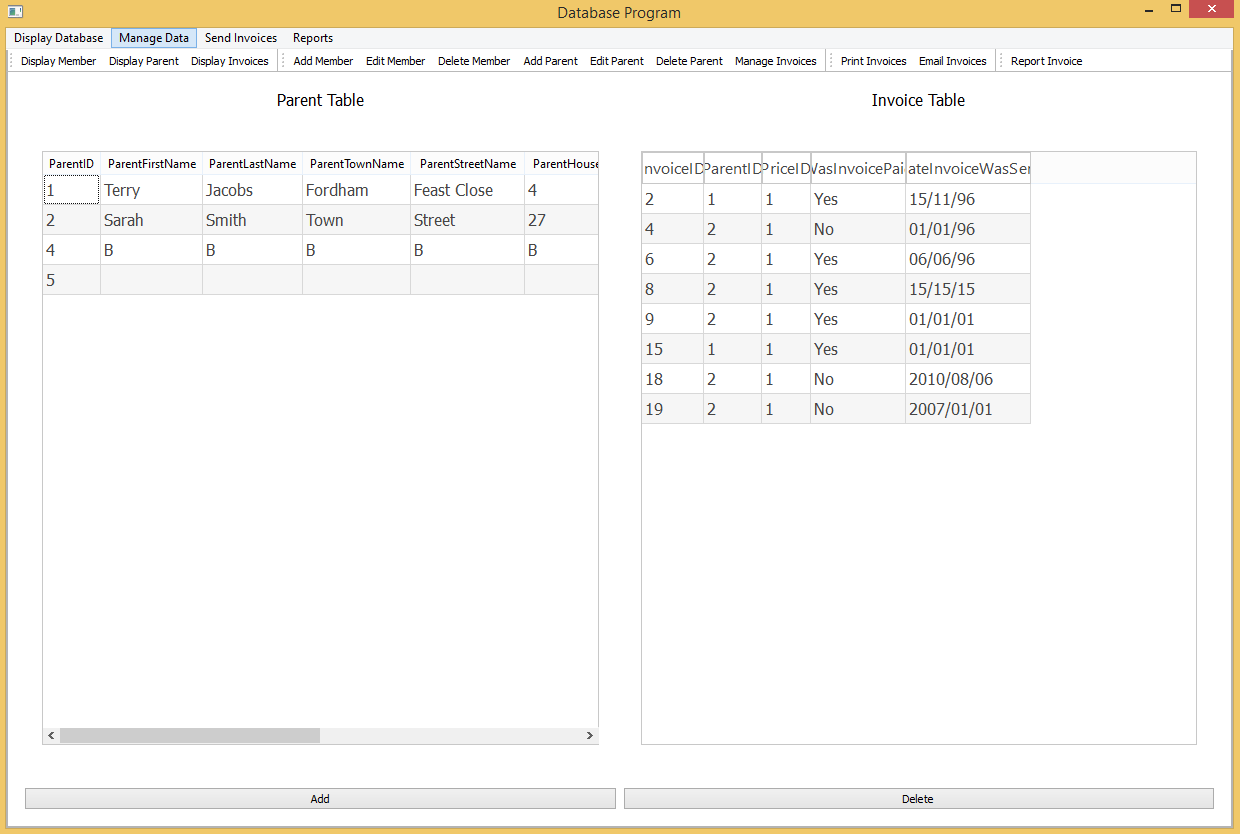
\includegraphics[width=\textwidth]{./Maintenance/Images/ManageInvoice.png}
    \caption{Managing Invoices} \label{fig:manage_invoice}
\end{figure}

Displays when Manage Invoices is clicked. Contains two tables, one showing the Parent table and one showing the Invoice table. Also contains two buttons, one to add an invoice one to delete invoices.

\begin{figure}[H]
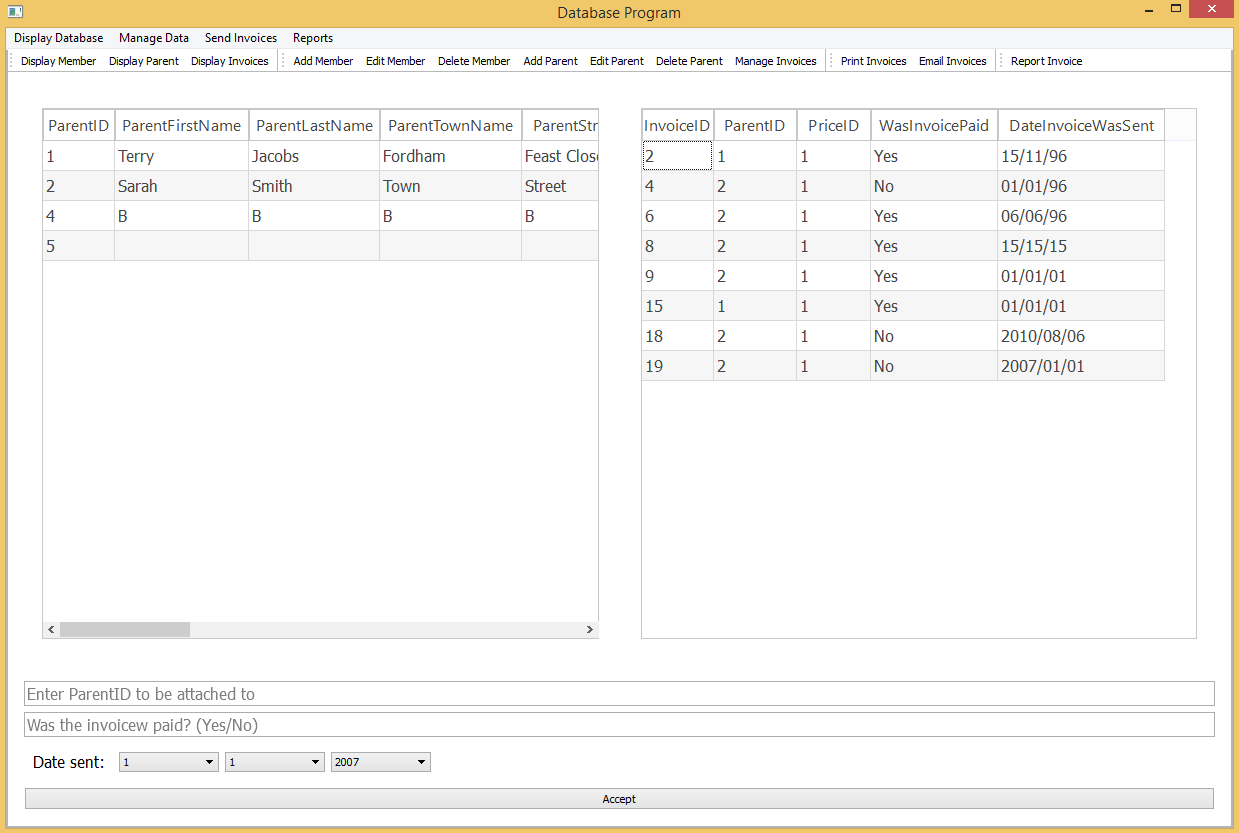
\includegraphics[width=\textwidth]{./Maintenance/Images/AddInvoice.png}
    \caption{Adding Invoice} \label{fig:add_invoice}
\end{figure}

Displays when Add is clicked. Contains a table view displaying the Invoice table and a series of linedits and comboboxes for the input of data into the table.

\begin{figure}[H]
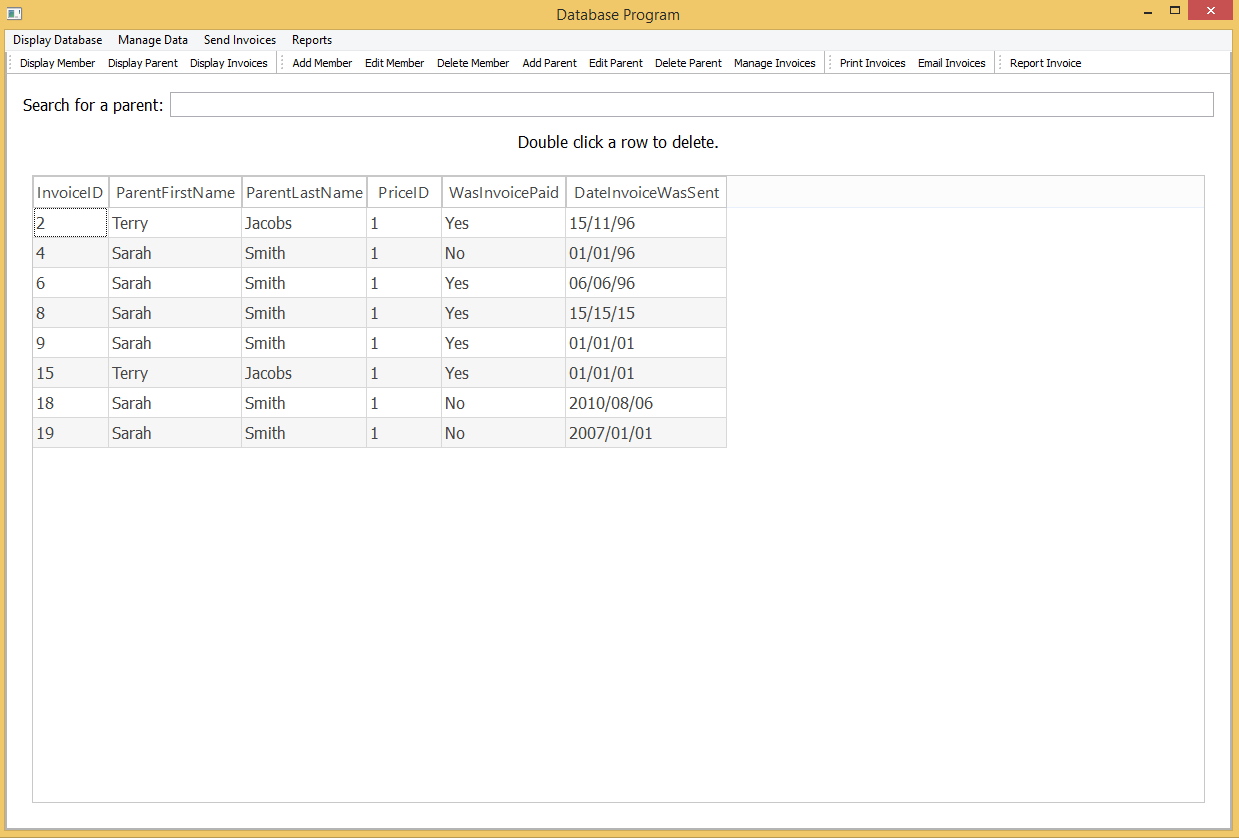
\includegraphics[width=\textwidth]{./Maintenance/Images/DeleteInvoice.png}
    \caption{Deleting Invoice} \label{fig:delete_invoice}
\end{figure}

Displays when Delete is clicked. Contains a table view displaying the Member table and a linedit to search the table.

\subsubsection{Reporting Invoices}
\begin{figure}[H]
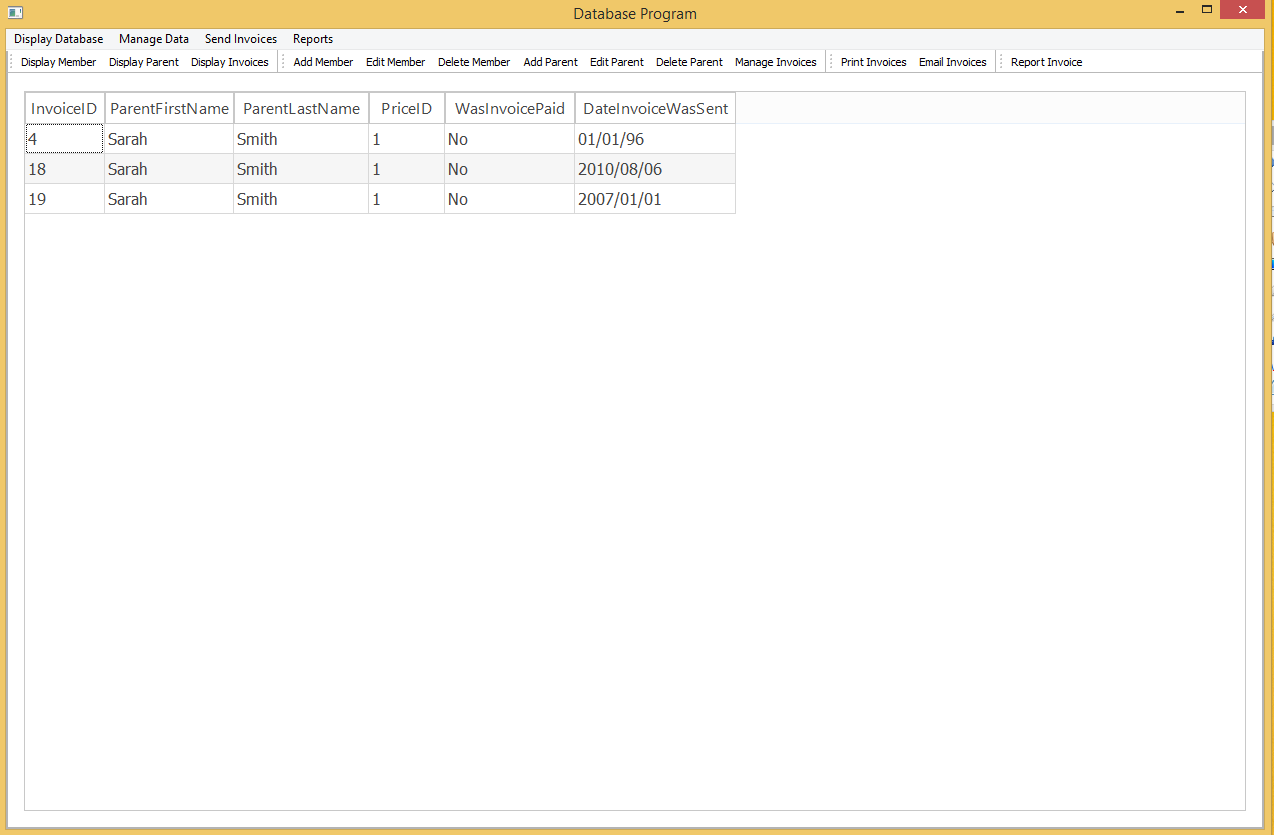
\includegraphics[width=\textwidth]{./Maintenance/Images/ReportInvoice.png}
    \caption{Reporting Invoice} \label{fig:report_invoice}
\end{figure}

Displays when Report Invoice is clicked. Contains a table view displaying the Invoices that have not been paid.

\subsection{ER Diagram}
\begin{figure}[H]
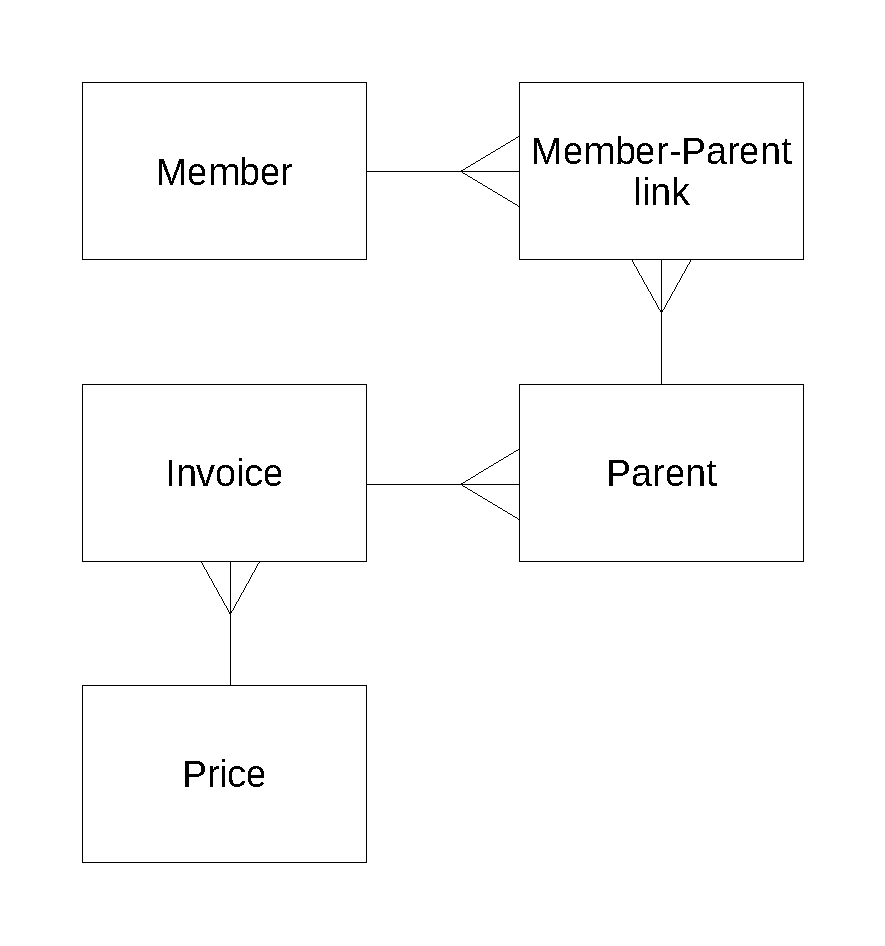
\includegraphics[width=\textwidth]{./Design/images/ER_diagram_design.pdf}
    \caption{ER diagram} \label{fig:ER_diagram}
\end{figure}

\subsection{Database Table Views}

\subsubsection{Member Table}
\begin{figure}[H]
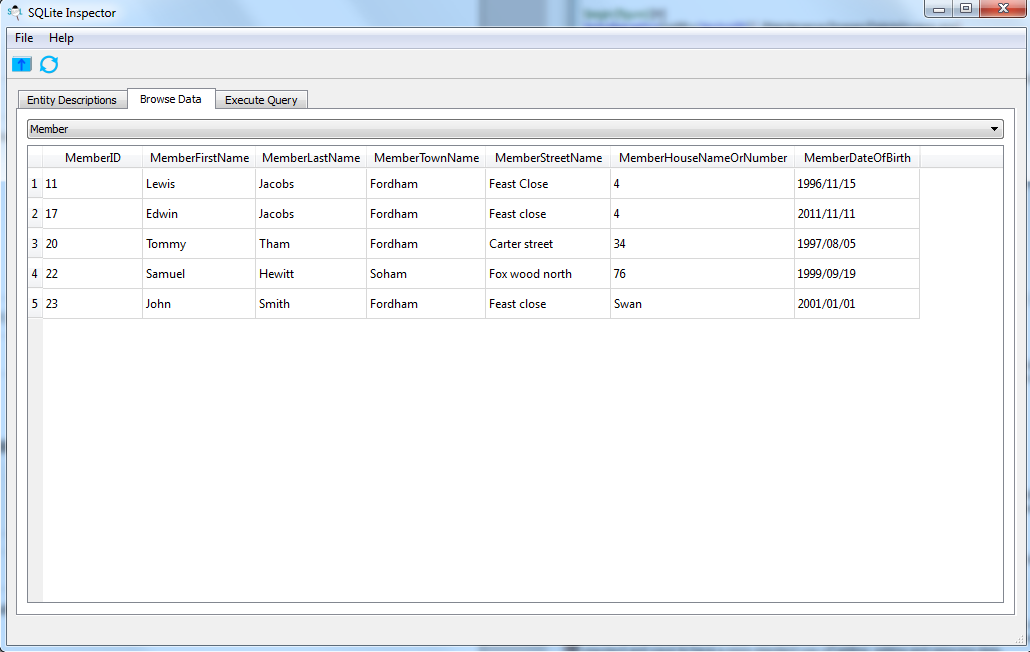
\includegraphics[width=\textwidth]{./Maintenance/Images/DatabaseMember.png}
    \caption{Member Table} \label{fig:member_table}
\end{figure}

\subsubsection{Parent Table}
\begin{figure}[H]
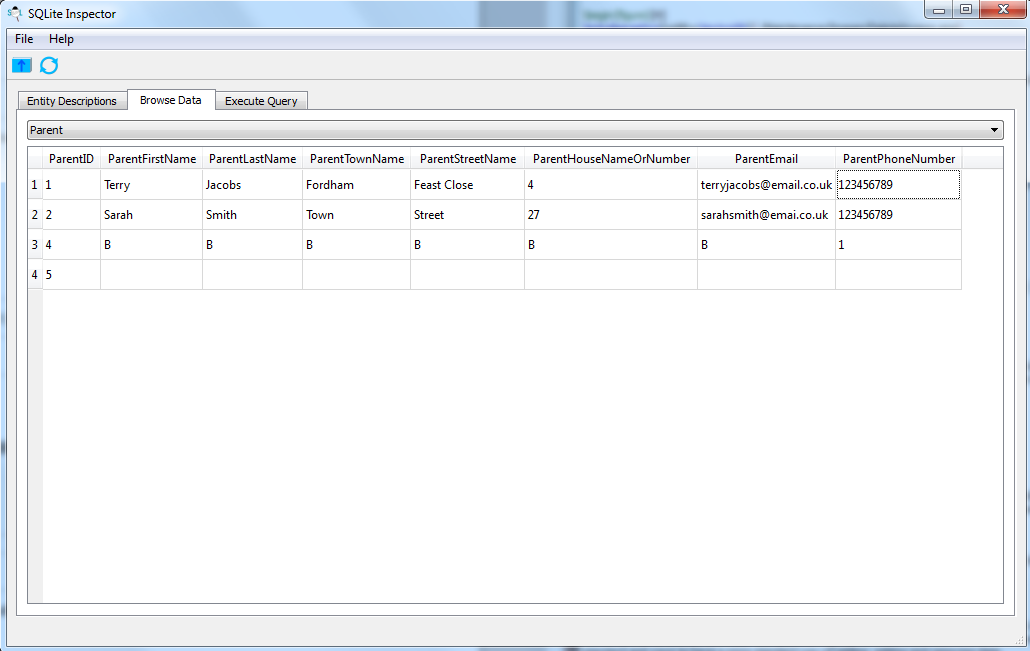
\includegraphics[width=\textwidth]{./Maintenance/Images/DatabaseParent.png}
    \caption{Parent Table} \label{fig:parent_table}
\end{figure}

\subsubsection{Invoice Table}
\begin{figure}[H]
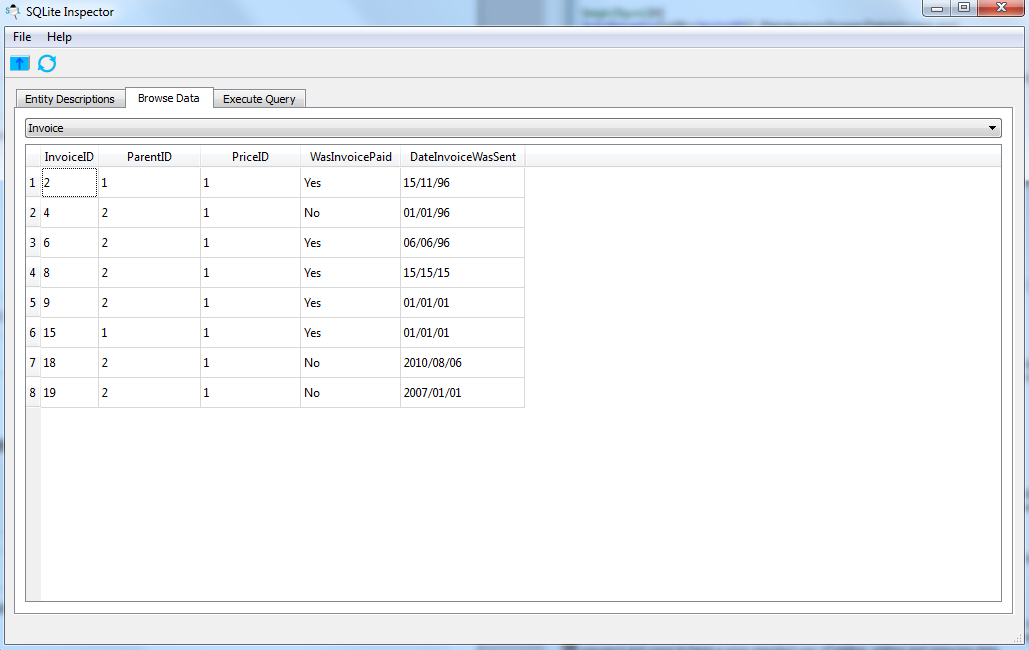
\includegraphics[width=\textwidth]{./Maintenance/Images/DatabaseInvoice.png}
    \caption{Invoice Table} \label{fig:invoice_table}
\end{figure}

\subsubsection{Price Table}
\begin{figure}[H]
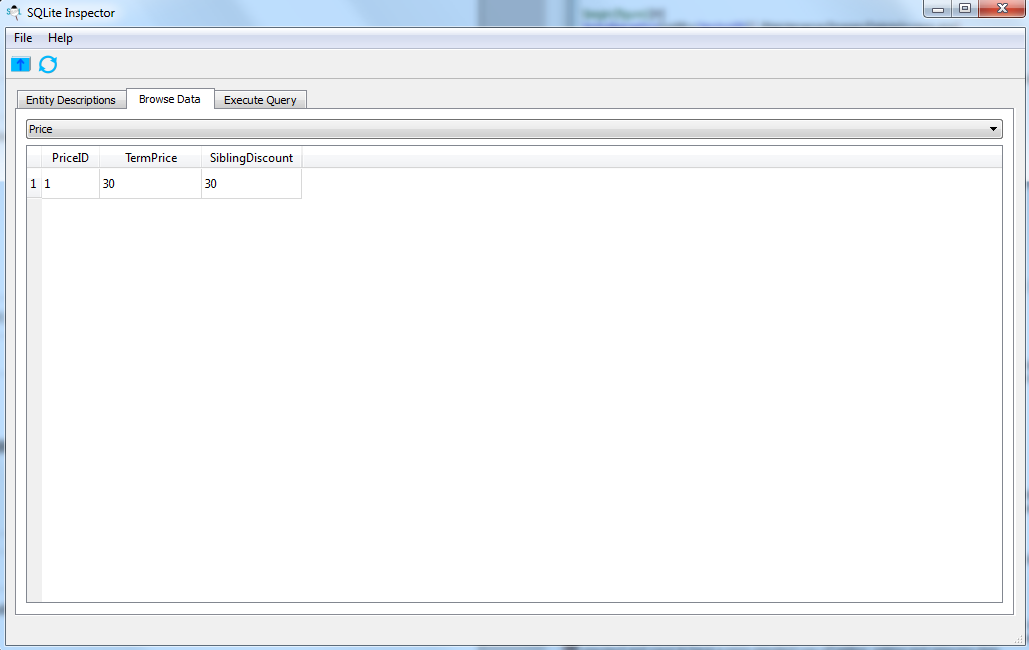
\includegraphics[width=\textwidth]{./Maintenance/Images/DatabasePrice.png}
    \caption{Price Table} \label{fig:price_table}
\end{figure}

\subsubsection{Connection Table}
\begin{figure}[H]
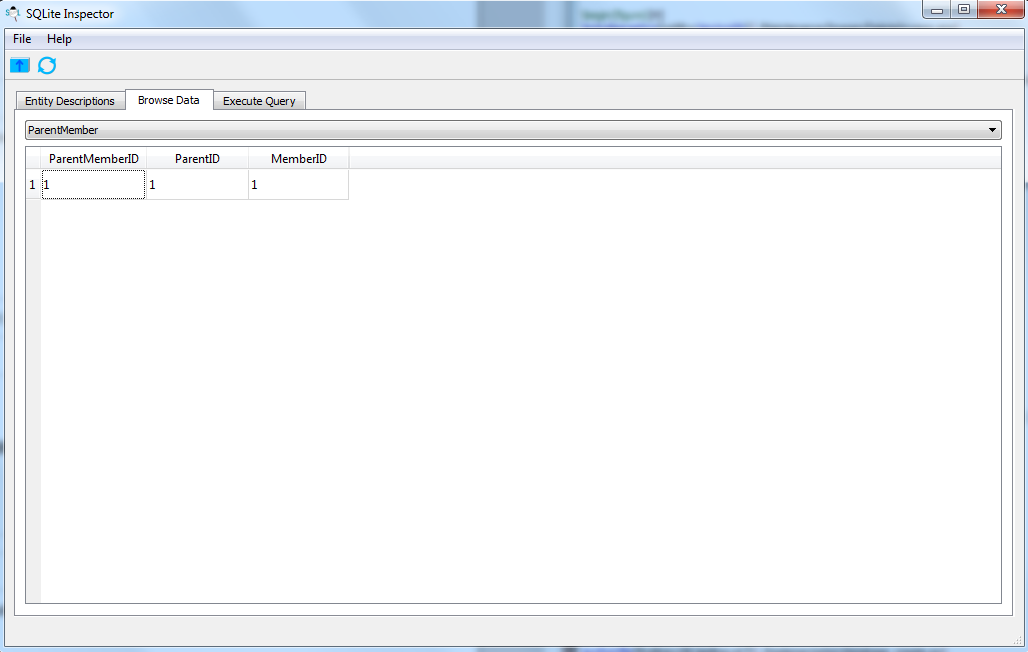
\includegraphics[width=\textwidth]{./Maintenance/Images/DatabaseParentMember.png}
    \caption{Connection Table} \label{fig:connection_table}
\end{figure}
 
The connection table was unused in the final version of the program.

\subsection{Database SQL}

\pythonfile[firstline=58,lastline=67]{./Implementation/database_create.py}

This SQL query and similar queries are in database\_create and are used to create the initial database. It creates a table of  Invoice that has the columns InvoiceID,ParentID,PriceID,WasInvoicePaid and DateInvoiceWasSent, while describing what data they can hold and what the primary key is, in this case InvoiceID. Line 8 and 9 set foreign keys of the columsn ParentID and MemberID while describing where they are located.

\subsection{SQL Queries}

From SQLConnection:

\pythonfile[firstline=56,lastline=66]{./Implementation/SQLConnection.py}

This SQL statement displays a table that shows the normal Invoice table but with the `ParentID' column replaced by the `ParentFirstName' and `ParentLastName' columns from the Parent table. Additionally, the data is filtered so only those where WasInvoicePaid is equal to `No' are displayed.

\pythonfile[firstline=84,lastline=84]{./Implementation/SQLConnection.py}

This SQL statement is used to select all the data from Member ordered by the column name, for example MemberFirstName and the type of order, for example ascending or desending.

\section{Testing}

\subsection{Summary of Results}
Rigourous testing reveals that although my system has a few flaws, it does mostly do what I intended it to do. However, while doing the testing I have noticed many area that could easy be made more effiencent or more user friendly, and ways to make my code cleaner and more sensical. Additionally, I have noticed many ways I could improve my program to a more professional standard and ways to have a more standard way of adding, editing and removing data.

The system meets many of the requirements from my client, although I did not have time to implement a way to print invoices effectively or a way to email invoices. However, emailing invoices was never part of my design specification.

Below are my results from my testing:

\begin{center}
    \begin{longtable}{|p{2cm}|p{5cm}|p{8cm}|}
        \hline
        \textbf{Test Series} & \textbf{Test Data} & \textbf{Actual Result}\\ \hline
        1.10 & John & The field is green \\ \hline
        1.11 & 12345 &  The field is red \\ \hline
        1.12 & John19 &  The field is red \\ \hline
        1.13 & J &  The field is green \\ \hline
        1.14 & John Smith & The field is green \\ \hline
        
        1.20 & Smith &  The field is green \\ \hline
        1.21 & 12345 &   The field is red \\ \hline
        1.22 & Smith19 &  The field is red \\ \hline
        1.23 & S &  The field is green \\ \hline
        1.24 & John Smith & The field is green \\ \hline
        
        1.30 & Fordham &  The field is green \\ \hline
        1.31 & Walton-on-the-Naze &  The field is green \\ \hline
        1.32 & Bury St Edmunds &  The field is green \\ \hline
        1.33 & Soham19 &  The field is red \\ \hline

        1.40 & Market-Street &  The field is green \\ \hline
        1.41 & Feast Close & The field is green \\ \hline
        1.42 & Church Street19 & The field is red \\ \hline
        
        1.50 & Swan & The field is green \\ \hline
        1.51 & Swan House & The field is green \\ \hline
        1.52 & 4 & The field is green \\ \hline
        1.53 & Swan 4 & The field is green \\ \hline
        
        \rowcolor{darkgrey} 1.60 & 15th November &  \\ \hline
        \rowcolor{darkgrey} 1.61 & 15/11/96 & \\ \hline
        \rowcolor{darkgrey} 1.62 & 15/11/1996 &  \\ \hline
        \rowcolor{darkgrey} 1.63 & 15.11.96 & \\ \hline
        
        \rowcolor{darkgrey} 1.70 & 1st January &  \\ \hline
        \rowcolor{darkgrey} 1.71 & 01/01/11 &  \\ \hline
        \rowcolor{darkgrey} 1.72 & 01/01/2011 &  \\ \hline
        \rowcolor{darkgrey} 1.73 & 05.01.11 & \\ \hline
        
        2.10 & Sarah & The field is green \\ \hline
        2.11 & 12345 & The field is red \\ \hline
        2.12 & Sarah19 & The field is red\\ \hline
        2.13 & S & The field is green\\ \hline
        2.14 & Sarah Smith &  The field is green\\ \hline
        
        2.20 & Smith & The field is green \\ \hline
        2.21 & 12345 & The field is red \\ \hline
        2.22 & Smith19 & The field is red \\ \hline
        2.23 & S & The field is green \\ \hline
        2.24 & Sarah Smith & The field is green \\ \hline
        
        2.30 & Fordham & The field is green \\ \hline
        2.31 & Walton-on-the-Naze & The field is green \\ \hline
        2.32 & Bury St Edmunds & The field is green \\ \hline
        2.33 & Soham19 & The field is red \\ \hline

        2.40 & Market-Street & The field is green \\ \hline
        2.41 & Feast Close & The field is green \\ \hline
        2.42 & Church Street19 & The field is red \\ \hline
        
        2.50 & Swan & The field is green \\ \hline
        2.51 & Swan House & The field is green \\ \hline
        2.52 & 4 & The field is green \\ \hline
        2.53 & Swan 4 & The field is green \\ \hline
        
        2.60 & 01234 & The field is amber \\ \hline
        2.61 & 01234567891 & The field is green \\ \hline
        2.62 & one two three & The field is red \\ \hline
       
        2.70 & johnsmith.co.uk & The field is amber \\ \hline
        2.71 & johnsmith@longroad.ac.uk & The field is green \\ \hline
        2.72 & johnsmithatlongroad.ac.uk & The field is amber \\ \hline
        
        3.10 & John & The correct entities are returned \\ \hline
        3.11 & Smith & The correct entities are returned \\ \hline
        3.12 & John Smith &  No entities are returned \\ \hline
        3.13 & 11 & No entities are returned \\ \hline
        
        4.10 & Click Accept button & The entity is added \\ \hline
        
        4.20 & Click Accept button & The entity is added \\ \hline
        
        5.10 & Left-click Display Member button & The Display Member screen is shown \\ \hline
        5.11 & Left-click Add Member button & The Add Member screen is shown \\ \hline
        5.12 & Left-click Print Invoices button & Invoice can be chosen and printed \\ \hline
        5.13 & Right-click Display Member button & No effect \\ \hline
        
        6.10 & Resize the main window & The window is resizable \\ \hline
        6.11 & Resize a pop-up window & The window is resizable\\ \hline
        
        6.20 & Check data in the tables is displayed correctly & The data is displayed under the right columns \\ \hline

       \rowcolor{lightgrey} 7.10 & Double click a member to delete & Entitiy is deleted \\ \hline
       \rowcolor{lightgrey} 7.11 & Single click a member to delete & Entitiy is selected \\ \hline
       \rowcolor{lightgrey} 7.12 & Double click outside of the table & No effect \\ \hline

       \rowcolor{lightgrey} 7.20 & Double click a parent to delete & Entitiy is deleted \\ \hline
       \rowcolor{lightgrey} 7.21 & Single click a parent to delete & Entitiy is selected\\ \hline
       \rowcolor{lightgrey} 7.22 & Double click outside of the table & No effect \\ \hline
        
       \rowcolor{lightgrey} 8.10 & Single click a field and type new data & New data us inserted into field \\ \hline
       \rowcolor{lightgrey} 8.11 & Double click a field and type new data & The entity is deleted \\ \hline
       \rowcolor{lightgrey} 8.12 & Single click outside of the table & The field that was last clicked will be edited \\ \hline
        
       \rowcolor{lightgrey} 8.20 & Single click a field and type new data &  New data us inserted into field \\ \hline
       \rowcolor{lightgrey} 8.21 & Double click a field and type new data & The entity is deleted \\ \hline
       \rowcolor{lightgrey} 8.22 & Single click outside of the table & The field that was last clicked will be edited \\ \hline

       \rowcolor{lightgrey} 9.10 & Left click report invoices button & The Report Invoices screen is shown \\ \hline
       \rowcolor{lightgrey} 9.11 & Right click report invoices button & No effect \\ \hline
    \end{longtable}
\end{center}

The orignal table can be found in my testing section on page \pageref{testing_section}

\subsection{Known Issues}
My testing highlighted some flaws in my program. Included in these flaws is the fact that data can be deleted from almost anywhere with no warning when a row is double clicked, when data should only be deletable from the DeleteMember, DeleteParent and DeleteInvoice screens. Additionally, I had some minor issues with validation but these will not impact the reilabilty of the program, however data is more likely to be entered incorrectly.

\section{Code Explanations}

\subsection{Difficult Sections}

\subsubsection{Creating a table in a database}
\pythonfile[firstline=3,lastline=22]{./Implementation/database_create.py}

A combination of sql and python code, this function attempts to create a new table. It opens a database as `db', and if the table being created already exists the user will be asked whether they want to overwrite the table. If the answer is yes or the table does not already exist then a new table is created. 

\subsubsection{Creating a table}
\pythonfile[firstline=34,lastline=41]{./Implementation/DisplayWidget.py}

This function creates a new QSqlTableModel as long as the current model is not also a QSqlTableModel. Then, it sets the table to the table passed into the function in the variable tableName, which is a string. Then the model is set to results\_table, the columns are resized to the contents of the table so all data is visible and the table is shown.

\subsubsection{Printing an invoice}
\pythonfile[firstline=85,lastline=93]{./Implementation/SendInvoices.py}

This function first gets the invoice template as a html. The QPrinter is created and the QPrintDialog is created with the printer.  Then, when the print dialog is executed the document is created with the html and the document is printed.

\subsection{Self-created Algorithms}

\subsubsection{Deleting data}
\pythonfile[firstline=501,lastline=503]{./Implementation/main_window.py}

While a very small piece of code, this allows a very intuitive way to delete data and an easy way to delete large quantities of data. With a small amount of extra code it could easily be made less llikely to wrongfully delete data.


\section{Settings}

Python, PyQt and SQL must be installed on the user's computer. The username and password will be set when the program is run for the first time, so care must be taken to make them both memorable.

\section{Acknowledgements}

I have no acknowledgements, all code and information is my own, that I am aware of.

\section{Code Listing}
\begin{landscape}
%include as many subsections as you have modules
\subsection{main\_window}

\label{main_window}
\pythonfile{./Implementation/main_window.py}

\subsection{database\_create}

\label{create_database}
\pythonfile{./Implementation/database_create.py}

\subsection{DisplayWidget}

\label{display_widget}
\pythonfile{./Implementation/DisplayWidget.py}

\subsection{SQLConnection}

\label{sql_connection}
\pythonfile{./Implementation/SQLConnection.py}

\subsection{AddData}

\label{add_data}
\pythonfile{./Implementation/AddData.py}

\subsection{EditData}

\label{edit_data}
\pythonfile{./Implementation/EditData.py}

\subsection{DeleteData}

\label{delete_data}
\pythonfile{./Implementation/DeleteData.py}

\subsection{ManageInvoices}

\label{manage_invoices}
\pythonfile{./Implementation/ManageInvoices.py}

\subsection{SendInvoices}

\label{send_invoices}
\pythonfile{./Implementation/SendInvoices.py}

\subsection{LoginBox}

\label{login_box}
\pythonfile{./Implementation/LoginBox.py}

\subsection{Password}

\label{password}
\pythonfile{./Implementation/Password.py}

\subsection{SearchingData}

\label{searching_data}
\pythonfile{./Implementation/SearchingData.py}

\subsection{SortingTable}

\label{sorting_table}
\pythonfile{./Implementation/SortingTable.py}

\subsection{StyleSheet}

\label{style_sheet}
\pythonfile{./Implementation/StyleSheet.py}

\end{landscape}
